% !TeX root = ../Book3.tex
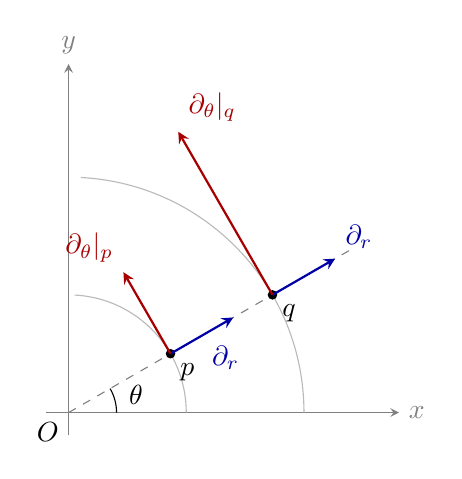
\begin{tikzpicture}[scale=1.15,>=stealth]
	\draw[->,gray] (-0.25,0)--(3.65,0) node[right]{\(x\)};
	\draw[->,gray] (0,-0.25)--(0,3.85) node[above]{\(y\)};
	\draw[gray!55] (0:1.3) arc[start angle=0,end angle=87,radius=1.3];
	\draw[gray!55] (0:2.6) arc[start angle=0,end angle=87,radius=2.6];
	\draw[dashed,gray] (0,0)--(30:3.6);
	\draw (0.53,0) arc[start angle=0,end angle=30,radius=0.53];
	\node at (15:0.77){\(\theta\)};
	\coordinate (P) at (30:1.3);
	\coordinate (Q) at (30:2.6);
	\fill (P) circle (1.5pt) node[below right]{\(p\)};
	\fill (Q) circle (1.5pt) node[below right]{\(q\)};
	\draw[->,thick,blue!65!black] (P)--++(30:0.8) node[midway,below right]{\(\partial_r\)};
	\draw[->,thick,blue!65!black] (Q)--++(30:0.8) node[above right]{\(\partial_r\)};
	\draw[->,thick,red!65!black] (P)--++(120:1.04) node[above left]{\(\partial_\theta|_p\)};
	\draw[->,thick,red!65!black] (Q)--++(120:2.08) node[above right]{\(\partial_\theta|_q\)};
	\node[below left] at (0,0){\(O\)};
\end{tikzpicture}
